\section {Properties the Protocol Garantees}
\label{chp:properities}

\subsection{Permissionless Property}
\dprotocol is a decentralized layer that anyone can join the network to help synchronize cross-chain bundled transactions. To prove permissionless, we need to show that although any running node can play the role of performing multi-blockchain transactions, the data stored in the chain is consistent and all local data in distributed nodes converge.

Given a group of bundled transactions $\mathbb{T} = \left\{tx_i\right\}$ submitted simultaneously, a valid trace from a start point of global state $s$ is a sequence of global state $s_0=s, s_1, \cdots s_n = s'$. It is obvious that different orders of $tx_k$ from the same $\mathbb{T}$ can lead to different valid traces. Thus we need a consensus algorithm so that all attending nodes in the \dprotocol can vote for a unique block producer to generate a globally valid trace.

We use a Merkle tree to record all the valid voting nodes and pin the root hash of the Merkle tree in native blockchains. For a new node to register itself as a valid node, it needs to fire a register transaction on the aggregator chain and synchronize the root hash itself before the vote.

To vote a node, a voter needs to sign a voting message and send the signed voting message to the target it votes. Inside the message, it contains the Merkle root hash of all valid voters' and targets' public addresses. Once a node receives a sufficient amount of voting tickets it will produce a zero-knowledge proof which shows that the total number of tickets reaches two-thirds of the total number of voters and all of them has the correct Merkle root hash. 

As mentioned in Section \ref{chp:protocol-details}, after the winner node calculated the ZKP proof of all the received signatures, it can start producing a block that represents a valid sequence of bundled transactions $\mathbb{T}$. This process is executed locally and the block producer can pick any order of $tx_i$ in the final sequence as long as it can generate a ZKP proof of the simulation.

\begin{figure}[!ht]
\begin{center}
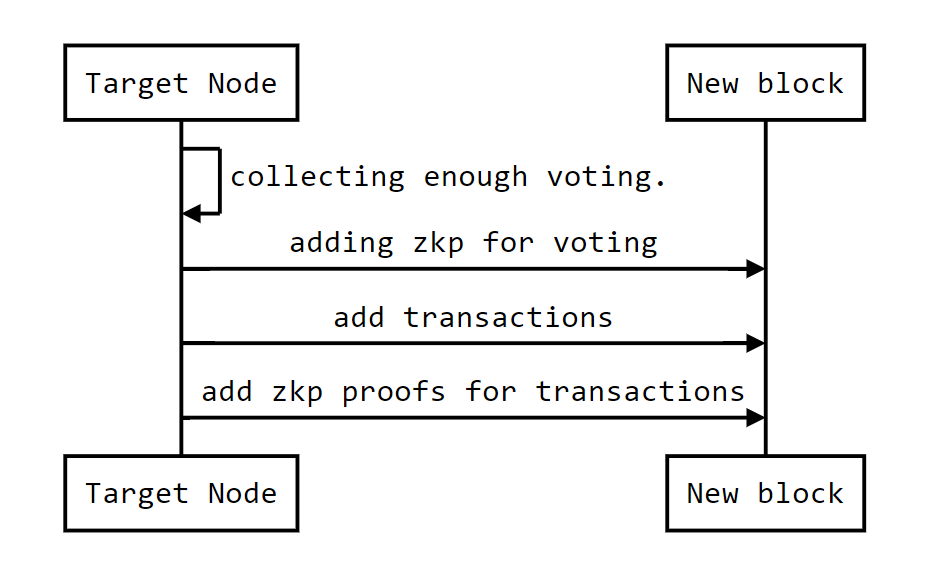
\includegraphics[scale=0.4]{produce-block.png}
\end{center}
\caption{Produce a block after voting}
\label{produce-block}
\end{figure}

Once the block is generated, it needs to be sent to the native blockchains $C_i$ to finalize before it can be recorded in the \dprotocol chain ledger. 

As the consensus algorithm solves the ordering problem, it remains to make sure the winner node can not produce a partially finalized block (finalize the block to a subset of the native blockchains). Thus we need a strategy to continue finalizing the block even if the winner node quit after generating the block. To achieve this, we simply record the proof data on the native chain $C_i$ during finalization so that if a block is synchronized partially, then all \dprotocol nodes will notice the recorded proof and can continue broadcasting the proof until it is fully synchronized. Moreover, if the winner does not finalize its block to any of the native chains, then we rely on the liveness property to make sure another block generator can be voted (see Section \ref{chp:sub:liveness}).

\subsection{Liveness Property}
\label{chp:sub:liveness}
We abstract the state transition diagram as follows (see Figure \ref{state-transition}), and we would like to show that all intermediate states lead to either a full finalize state or skip state.
\begin{figure}[!ht]
\begin{center}
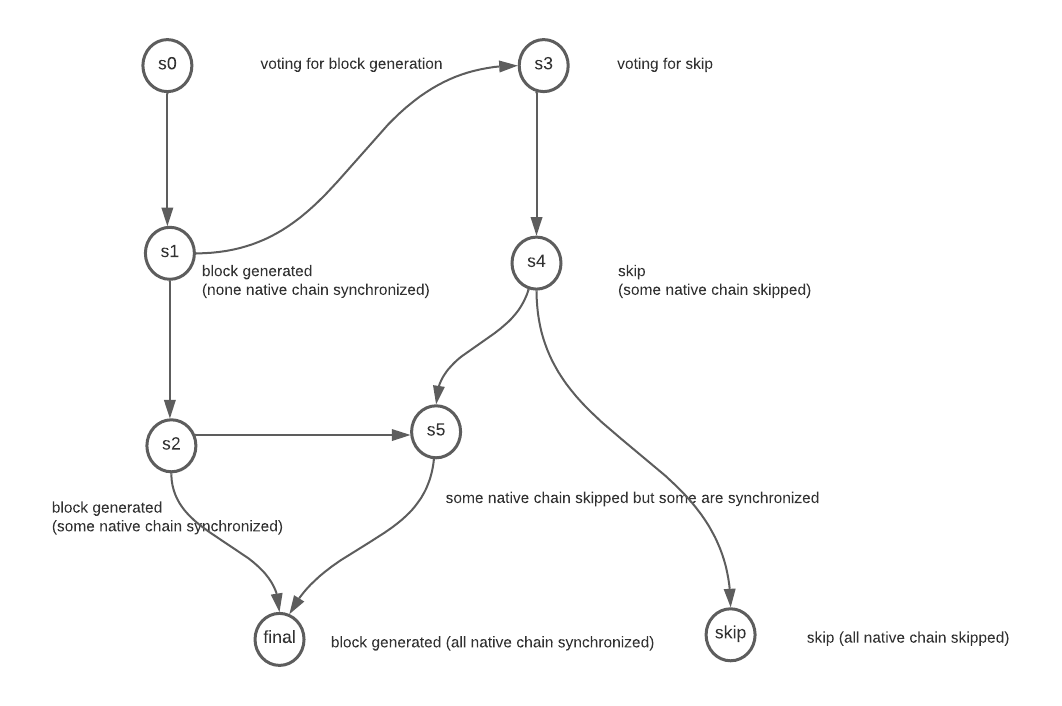
\includegraphics[scale=0.2]{state-transition.png}
\end{center}
\caption{State transition}
\label{state-transition}
\end{figure}

%then the voter needs to trigger another vote to skip the current round of block producing and send the skip signal to all native blockchains. Once all the native blockchains received the skip signal, they will not accept any block with the current round number and the next round of block generation can start. If one of the native blockchains received the synchronizing call of the generated block, then all the nodes need to perform a revoke-skip vote so that they can revoke the skip signal on native blockchains.

Notice that in the protocol, the interesting state is $s_4$ in which the block is generated and some nodes may suspected that the finalizing stage is halted and vote to skip the current round. If any of the node notice that the block is partially finalized on a subset of native blockchains then it leads to $s_5$ and there is no need to skip. Otherwise, the current round is skipped. Thus the final state of all native-block chains converges to the same state.

\subsection{Safety Property}
Recall that for a bundled transaction $tx = {tx_i}$, the safety property of a protocol to carry out $tx$ is that either all $tx_i$ succeed or none of them succeed. Below we discuss the safety property of \dprotocol in three scenarios.

%First, we show that the safety property holds if a transaction $tx$ does not have an invoke transaction or any side effects. Second, we further prove that if all side effects are safe then the safety property still holds. Finally, we show that if the first transaction of a bundled transaction $tx$ is an invoke transaction, then we can rely on our liveness property to ensure that if the invoke transaction succeeds then all sub transactions in $tx$ will eventually be finalized.

%and if the invoke transaction fails then it can be revoked using a revoke transaction so that the global state stays the same. \\

\smallskip\noindent\emph{1. Bundled transaction with no invoke transaction}\\
If a bundled transaction does not start with an invoke transaction, then it means the bundled transaction is invoked directly on the aggregator chain. Because all components $tx_i$ of $tx$ are simulated and performed on the aggregator chain and a proof of the execution of $tx$ can not be generated if any $tx_i$ fails during the simulation, a transaction can only be executed as a whole. Thus the safety properties hold naturally.

%If the proof is valid and is submitted to native chains then it will pass the validation check and then we expect that the local state of the native chain will change accordingly with no exception.

%Since the liveness property promises that all native chains will eventually receive the valid proof, it remains to show that the state updating protocol in our proxy contract is safe.

%A smart contract is a piece of code that can not be changed once deployed, its behavior is fixed and predictable. Thus we can assume that our proxy contract always performs correctly according to its pre-defined functionality. Suppose that $s$ is the start global state, $tx$ is the transaction and $s'$ is the final state. When our proxy contract receives $MTH(s)$, $tx$, $MTH(s')$ and the state difference $\delta_{s}$ together with a zero-knowledge proof $p(MTH(s), MTH(s'), tx)$, our proxy contract will do the following:

%\begin{enumerate}[leftmargin=*]
%\item Proxy contract checks that pined local global hash equals $MTH(s)$. This makes sure that the current local state $s_i$ is consistent with the global state $s$.

%\item Proxy contract verifies the proof $p(s, s', tx)$. Once the verification succeeds, it can guarantee that $s'$ is a valid final state after simulating $tx$ over $s$.

%\item Compute the changes of $s_i$ and change the local state from $s_i$ to $(s_i)'$. Since updating the local state is a monadic function of the local state, it will never fail which means once the proof of $tx$ is verified, the local state will be changed correctly for sure.

%\item Proxy contract performs all the related side effects for each transactions $tx_k$ in bundled transaction $tx$. 
%\end{enumerate}

\smallskip\noindent\emph{2. Bundled transaction with side-effects.}\\
We notice that side effects is the only place where a finalizing call will fail even if the proof is correct. To address this problem, we break down side effects into two categories. The first category contains side effects like emitting events, logging, or pure history recording which are naturally safe since they will never fail by design. The second category includes unsafe function calls like assets transfer. This kind of unsafe function can still be safe if we perform sanity checks in $tx$.

For example, if $tx_k$ in $tx$ will trigger a side-effect $e_k$ and $e_k$ is safe under a condition $P$ where $P$ is a predicate of global state $s$, then we can insert a check after $tx_k$ as following:

\begin{code}
...
let s' = tx_k(s);
if !P_k(s'):
    raise Excepition(sanity check failure)
let s'' = tx_{k+1}(s);
...
\end{code}
Once $tx$ is modified so as above, a valid proof of a correct simulation of $tx$ will ensure not only the final state valid but all the sanity checks are all valid as well. Thus $e_k$ will be safe for sure.\\

\noindent\smallskip\emph{3. Bundled Transaction with an Invoke Transaction.}\\
If a bundled transaction $tx$ starts with an invoke transaction $tx_0$ on $C_i$, then this invoke transaction on chain $C_i$ triggers the execution of the bundled transaction $tx$ by emitting an invoking event. This event is reported to the aggregator chain through a native chain ZK monitor \cite{garoffolo2020zendoo}.

%The aggregator chain bundled transaction simulator relies on the honesty of the reporter and if the relayer is hacked it can exploit the protocol by reporting malformed results of the invoke transaction. For example, in the transfer scenario, if a report reports the wrong amount of assets that have been transferred from Alice to Bob in Chain A then a successfully finalized $tx$ will trigger a wrong transfer from Bob to Alice on Chain B.

%To address this problem and make sure the protocol is safe even though the relayer is dishonest,
In this scenario, we split the process of the changes of global state $s$ into two stages. At the first stage $s$ is changed to $s'$ after invoke transaction and at the second stage $s'$ is changed to $s''$ after the whole simulation of $tx$.

During the first stage, $s'$ is pinned in native chain $C_i$ once the invoke transaction is executed and the second stage is encoded by a zero-knowledge proof generated from \dprotocol node. During the finalization, the proof of $tx$ now encodes the proof from $s'$ to $s''$.

%To ensure that the invoke transaction $tx_0$ is reported correctly, the verifier only needs to compare the MTH of the local calculation of $s'$ and the hash provided by the aggregator chain Node. If the hash is the same, then it means $tx_0$ is reported honestly. Moreover since $s'$ are checked, $s''$ can be treated as a valid simulation from $s$ to $s''$. In conclusion, the finalization steps are listed as follows:

%\begin{enumerate}[leftmargin=*]
%\item Proxy contract checks that pined local global hash equals $MTH(s'')$. This makes sure that the current local state $s_k^i$ is consistent with the global state $s'$ after processing invoke transaction. Thus the invoke transaction are reported honestly.

%\item Proxy contract verifies the proof $p_{t}(s', s'', tx)$. Once the verification succeeds, it can guarantee that $s''$ is a valid final state after simulating $tx$ over $s$.

%\item Compute the changes of $(s^i)'$ and change the local state from $(s^i)'$ to $(s_i)''$. Since updating the local state is a monadic function of the local state, it will never fail which means once the proof of $tx$ is verified, the local state will be changed correctly for sure.

%\item Proxy contract performs all the related side effects for each transactions $tx_k$ in bundled transaction $tx$. 
%\end{enumerate}

\subsection{Linearizability Property}
In concurrent programming, an operation (or set of operations) is linearizable if it consists of an ordered list of invocation and response events. Since in each block generation round only one node wins the right to produce a block, the linearizability hold if and only if the final state simulated in the block can be represented as a sequence of bundled cross transactions $\{tx_i\}$. Since each block producer needs to create a zero-knowledge proof to show that $s' = tx_k \circ tx_{k-1} \circ \cdots tx_0(s)$ (where $\circ$ is function composition), a valid proof already shows the linearizability property. Thus in \dprotocol protocol, the linearizability property holds trivially. 
